\chapter{MARCO TEÓRICO }

En el presente capítulo se abordarán los temas más importantes que servirán como base para el desarrollo del proyecto. En particular, se explicarán los fundamentos de los sistemas de recomendación, haciendo enfasis en los diferentes enfoques y técnicas más utilizadas en este campo. Además, se presentará una revisión detallada de los algoritmos de Búsqueda de Vecinos, cómo funcionan y las métricas que utilizan con el fin de entender a profundidad los algoritmos actuales como \textit{Voyager}, que será explicado en detalle al final del capítulo.

\section{FUNDAMENTOS DE LOS SISTEMAS DE RECOMENDACIÓN }

Los sistemas de recomendación son \textbf{agentes de información personalizada} que brindan sugerencias de elementos que \textit{podrían} ser útiles para un usuario.  Los resultados dados por un sistema de recomendación se denominan \textbf{Recomendaciones} que representan una opción valiosa que podría ser del interés de una persona o usuario.

\subsection[CONCEPTOS BÁSICOS]{CONCEPTOS BÁSICOS DE LOS SISTEMAS DE RECOMENDACIÓN }


Los Sistemas de Recomendación se fundamentan mediante entidades que aportan información desde diferentes medios:

\begin{itemize}
    \item \textbf{Usuario: } La entidad a la que se le hacen llegar las recomendaciones es denominada como \textit{usuario}. 
    \item \textbf{Items: } Es una pieza de información que refiere a un objeto tangible o digital que el sistema de recomendación sugerirá al usuario en una interacción a través de la Web, email o mensajes de texto \parencite{Kotkov2020Serendipity}.
    \item \textbf{Fuente de Conocimiento: } Determina qué técnica será usada para definir el medio de información y determinar el conocimiento necesario para brindar sugerencias relevantes.
\end{itemize}

El principio básico que fundamenta a los algoritmos de recomendación es la dependencia significativa que existe entre un \textit{usuario} y los \textit{items} con los que interactúa.

\subsection[OBJETIVOS GENERALES]{OBJETIVOS DE UN SISTEMA DE RECOMENDACIÓN: }

Según \parencite{Aggarwal2016} más allá de los objetivos mercadológicos que se le atribuyen a los sistemas de recomendación enfocados en mejorar el rendimiento económico de una plataforma, se pueden definir objetivos técnicos y operacionales que mejoran el rendimiento de un sistema en éste ámbito.

\begin{itemize}
    \item \textbf{Relevancia: }Un sistema de recomendación siempre debe brindar sugerencias relevantes para el usuario.
    \item \textbf{Novedad: }  Las recomendaciones suelen ser más útiles cuando sugieren elementos que el usuario no ha visto antes. Además, recomendar los objetos más populares puede conducir a reducir la diversidad del consumo.
    \item \textbf{Sorpresa: } No basta con que los objetos de recomendación sean nuevos para el usuario, sino que también deben sorprenderlo, dándole la sensación de un \textit{descubrimiento inesperado.}
    
    \item \textbf{Diversidad de Recomendaciones: } La lista de sugerencias obtenidas deben ser suficientemente diferentes entre sí para no aburrir al usuario, sin embargo, la diversidad de \textit{items} no debe alejarse demasiado de sus preferencias.
   \enquote{\textit{La diversidad tiene el beneficio de asegurar que el usuario no se aburre de constantes recomendaciones de items similares. }} [\cite{Aggarwal2016}]
\end{itemize}

\newpage

Existen dos versiones diferentes que definen los resultados esperados de un Sistema de Recomendación, ambos buscan resolver el problema de encontrar items relevantes para los usuarios mediante modelos distintos:


\begin{enumerate}
    \item \textbf{Versión de Predicción: } Se basa en predecir la calificación que el usuario daría a un item. Se asume que existe un conjunto de Datos de Entrenamiento que indica las preferencias del usuario.
    \item \textbf{Versión de Top - $k$: } Este enfoque argumenta que muchos de los sistemas no necesitan conocer la calificación estimada del usuario, por el contrario, solo necesitan saber qué recomendar sin necesidad de estimar una calificación exacta. Esto se suele hacer mediante un Top - $k$ elementos que probablemente le gusten al usuario.
\end{enumerate}

\subsection{PRINCIPALES ENFOQUES DE RECOMENDACIÓN }
Para que un sistema de recomendación logre cumplir los objetivos básicos esperados se necesita establecer de forma clara cuál será el filtro para sugerir items al usuario eligiendo diferentes enfoques que se adapten a los resultados que se buscan obtener.

Basándose en \parencite{ISINKAYE2015261} existen diferentes filtros de recomendación principales, sin embargo, se muestran los más relevantes para el presente proyecto:

\subsubsection[BASADO EN CONTENIDO]{ENFOQUE BASADO EN CONTENIDO }
Es una técnica de sistema de recomendación que se centra en el análisis de atributos de cada item para generar predicciones sobre las preferencias del usuario. Se apoya de valoraciones previamente vinculadas a un perfil que permiten identificar características clave de los objetos que el usuario ha calificado, principalmente de aquellos que cuentan con una valoración positiva.  Por esta razón, la eficacia de este enfoque se basa en la cantidad de información disponible de los items.

Los algoritmos que implementan esta técnica suelen basarse en modelos de análisis estadístico y de \textit{Machine Learning.}

\newpage

\textbf{VENTAJAS }
\begin{itemize}

    \item \textbf{Capacidad recomendar items nuevos: } Este enfoque permite sugerir elementos que aún no han sido evaluados por los usuarios gracias a la información contenida en sus \textit{metadatos} \footnote{\textbf{Metadatos: } Atributos que describen, proveen contexto, indican la calidad, o documentan las características de un objeto. \parencite{Greenberg09092005}}.
    \item \textbf{Alta adaptabilidad: } Se adapta a los cambios de preferencia del usuario en un lapso corto de tiempo.

    \item \textbf{Independencia entre usuarios: } Los usuarios reciben recomendaciones sin la necesidad de compartir su información con externos, priorizando la privacidad y seguridad de los datos.
    
\end{itemize}

\textbf{DESVENTAJAS }
\begin{itemize}

    \item \textbf{Dependencia en la profundidad de la información: } Los motores de recomendación basados en esta técnica son dependientes de los metadatos vinculados a los items. Por lo tanto, requieren que los elementos sean profundamente descritos por sus atributos. Esto es definido como \textbf{\textit{Análisis limitado al contenido}}.
    
    \item \textbf{Falta de Diversidad: } Es probable que las sugerencias sufran de \textit{sobre-especialización} o, en otras palabras, que carezcan de diversidad debido a que los usuarios están restringidos a obtener recomendaciones similares a los items asociados a sus perfiles.
\end{itemize}

\subsubsection[COLABORATIVO]{ENFOQUE COLABORATIVO}

A diferencia del enfoque basado en contenido, que se centra en los atributos de los items, el enfoque colaborativo se centra en las similitudes entre lo usuarios para generar recomendaciones.

Este enfoque funciona construyendo una base de datos descrita por una matríz \textit{usuarios - items} que representa la preferencia de un conjunto de usuarios por un item particular. Esto significa que vincula a diferentes perfiles con preferencias e intereses similares para guiar las recomendaciones, formando así un grupo  de perfiles que comparten intereses denominado \textit{Vecindario}. 


Por lo tanto, un usuario recibe recomendaciones de contenido que no ha evaluado pero que otros usuarios dentro de su \textit{Vecindario} han calificado de forma positiva. Los resultados que se pueden obtener a través de este enfoque son los siguientes:

\begin{itemize}
    \item \textbf{Predicciones: } Es un valor numérico que expresa un puntaje del elemento $j$ para el usuario $i$, esta predicción se representa con la notación $R_{i,j}$.
    \item \textbf{Rankings: } Es una lista de los Top - $N$ elementos que al usuario le podrían gustar más.
\end{itemize}

\begin{figure}[h!]
    \centering
    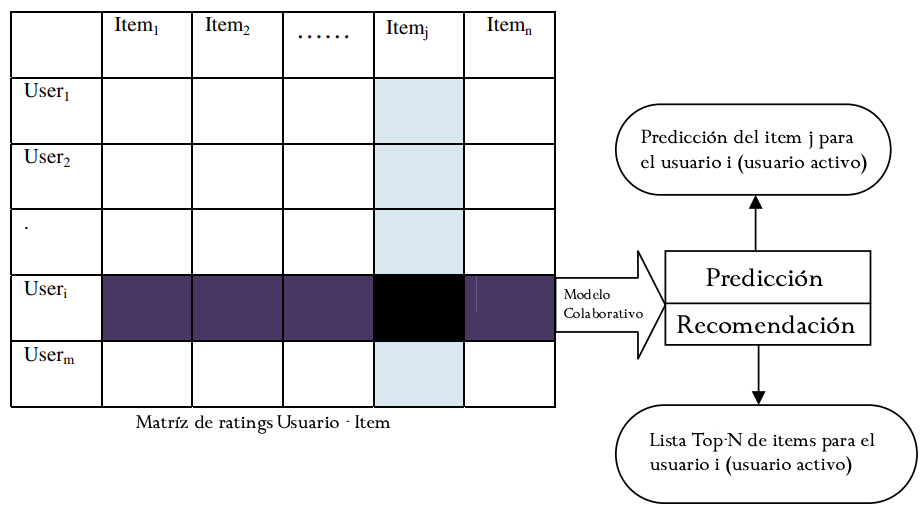
\includegraphics[width=0.7\linewidth]{FiltroBasadoenContenido.png}
    \caption{Ejemplo del Filtro Basado en Colaboración \parencite{ISINKAYE2015261}.}
    \label{fig:FiltroColaborativo}
\end{figure}

En la figura \ref{fig:FiltroColaborativo} se muestra un ejemplo de funcionamiento del enfoque colaborativo. Se puede observar que la matríz está compuesta por filas que representan a los usuarios de un mismo \textit{Vecindario}, y por columnas que representan a los \textit{items}. Las intersecciones mostradas de color morado representan la calificación que el usuario ha dado a elementos previos, y la intersección diferenciada de color negro expresa una predicción basada en las calificaciones que los vecinos han asignado a ese item.
El diagrama remarca la distinción entre \textit{Predicción} y la \textit{Recomendación} dado que, en el caso de la predicción,  la intersección representada en color negro representa el valor $R_{i,j}$, y en el caso de la recomendación representa un \textit{item} dentro de los Top - $N$ items del usuario actual.

\newpage

\textbf{VENTAJAS}

Este enfoque tiene ventajas fuertemente diferenciadas respecto al enfoque basado en contenido, algunos de sus puntos fuertes son los siguientes:

\begin{itemize}
    \item \textbf{Independencia al Contenido: } Los algoritmos colaborativos pueden funcionar de forma efectiva en dominios en los cuales no existe diversidad de información (o metadatos) para describir los items.
    \item \textbf{Recomendaciones basadas en Serendipia \footnote{\textbf{Serendipia en Sistemas de Recomendación: } \textit{Items} que son relevantes pero inesperados para el usuario. \textit{Items} que son nuevos e inesperados. \parencite{Kotkov2020Serendipity}} }: Significa que tiene la capacidad de recomendar elementos que son aparentemente ajenos a las preferencias del usuario, pero que para sus \textit{vecinos} son relevantes, conectando al usuario con contenido nuevo.
\end{itemize}

\textbf{DESVENTAJAS}

\begin{itemize}
    \item \textbf{Problema de \textit{Inicio Frío}}: Se refiere a la situación en donde el Sistema de Recomendación no tiene información adecuada acerca del usuario o acerca del item para hacer predicciones relevantes \parencite{Burke2007}. Este problema es crucial ya que este enfoque se vuelve dependiente de conocer con el tiempo las preferencias del usuario que, inicialmente, son desconocidas.

    \item \textbf{Problema del \textit{Esparcimiento de Datos}}: Otro de los puntos de los que depende el enfoque colaborativo es en las calificaciones hechas por los usuarios, causando la necesidad de que existan previas valoraciones para los items, de lo contrario, se generan recomendaciones poco relevantes.
    
    \item \textbf{Escalabilidad}: Un problema bastante común en los algoritmos de recomendación con enfoque colaborativo es la escalabilidad. Cuando la cantidad de usuarios e items crecen rápidamente, la complejidad computacional crece de forma lineal en relacion a estos dos aspectos, dando un costo computacional representado por la siguiente fórmula: $O(items \ \cdot \ usuarios)$\footnote{\textbf{Notación \textit{BIG O}:}  Es un estándar que describe el orden de crecimiento de un algoritmo en función del tamaño del problema. En el presente documento se usará para expresar la complejidad computacional de los algoritmos descritos.}. Es importante mencionar que un algoritmo lineal no logra ser eficaz cuando la cantidad de información es masiva.

    \newpage

    \item \textbf{\textit{Sinónimos: }} Se refiere a la situación en la que items muy similares aparecen registrados con diferentes nombres o identificadores \parencite{ISINKAYE2015261}. Los sistemas de colaboración no reconocen automáticamente que se trata de equivalencias; por ejemplo, \textit{item 1: Álbum Let It Be - The Beatles}, \textit{item 2: Álbum Let It Be (Remasterizado) - The Beatles}. En este caso, el sistema podría tratarlos como elementos completamente diferentes, a pesar de estar estrechamente relacionados.
\end{itemize}

\textbf{ENFOQUE HÍBRIDO}

A pesar de que los enfoques de recomendación basados en contenido y colaborativos son eficaces en escenarios particulares, sus desventajas inherentes limitan su escalabilidad en plataformas de uso masivo.  El enfoque híbrido busca solventar las desventajas de cada enfoque combinando diferentes técnicas de recomendación con el objetivo de evitar las limitaciones y problemas que los enfoques puros pueden enfrentar.

Los sistemas de recomendación híbridos están fuertemente relacionados al campo del \textit{Análisis de Conjuntos (Ensemble Analysis)} en los cuales se combina el poder de multiples tipos de algoritmos basados en \textit{Machine Learning} para crear modelos más robustos \parencite{Aggarwal2016}.  

\textbf{TÍPOS DE ENFOQUES HÍBRIDOS}
\begin{itemize}
    \item \textbf{Enfoque Híbrido basado en Pesos: } Este enfoque combina los resultados de diferentes enfoques de recomendación para crear una lista de recomendaciones que integran las calificaciones de cada técnica mediante una fórmula lineal. Inicialmente todas las técnicas usadas inician con un peso igualado que se modifica a través de la evaluación del usuario.
    \item \textbf{Enfoque Híbrido por Conmutación: } Este enfoque se basa en una heurística definida que selecciona la mejor técnica de recomendación adaptada al momento. Por ejemplo, si se necesita de un algoritmo de recomendación para un usuario nuevo, se puede identificar que usar el enfoque colaborativo no es una buena opción debido al \textit{Inicio Frío}, por lo tanto, se elige el enfoque basado en contenido. El beneficio de esta estrategia es que el sistema es sensible a las fortalezas y debilidades de sus enfoques de recomendación \parencite{ISINKAYE2015261}. 

    Sin embargo, esta conmutación de enfoques tiene una desventaja inherente debido al costo computacional que requiere el cambiar de métodos constantemente, principalmente por la diferencia de criterios y parámetros de información que cada enfoque requiere.

    \item \textbf{Enfoque Híbrido Combinado: } Este enfoque combina los resultados de diferentes algoritmos de recomendación, ejecutándolos en paralelo para generar una lista única de recomendaciones. El beneficio principal de esta estrategia es que el rendimiento local de un enfoque específico no suele afectar de manera significativa al rendimiento global del sistema, resultando en una mayor robustez.
    
\end{itemize}

\section[EVALUACIÓN DE UN SISTEMA DE RECOMENDACIÓN]{PARADIGMAS Y MÉTRICAS DE EVALUACIÓN PARA UN SISTEMA DE RECOMENDACIÓN: }

Los Sistemas de Recomendación deben desarrollarse mediante un enfoque alineado con los objetivos esperados respecto a la interacción con los usuarios. Estos objetivos principales han sido estudiados y seccionados en paradigmas de evaluación, sin embargo, basándose en la investigación de \parencite{Aggarwal2016} se pueden definir también métricas de evaluación generales para calificar el desempeño de un sistema de recomendación. En esta sección se mencionarán generalidades de los paradigmas de evaluación y se hará un enfasis en las métricas generales.

\subsection{PARADIGMAS DE EVALUACIÓN: }

Existen tres paradigmas de evaluación principales dirigidos a los sistemas de recomendación, donde las principales diferencias se centran en cómo los usuarios interactúan con las métricas de evaluación.

\begin{enumerate}

    \item \textbf{Usuarios de Estudio: } Este paradigma se centra en invitar a los usuarios a un proceso de evaluación para interactuar con el sistema y evaluar su desempeño en contextos específicos. Por lo tanto, las mediciones se obtienen de los comentarios de los usuarios y de las observaciones de interacción obtenidas  por el sistema. 
    Esta información se usa para entender cuáles fueron las preferencias del usuario, qué le gustó y qué no le gustó.

    La principal ventaja de este paradigma es que los usuarios dan permisos explícitos para usar su información en función de la evaluación del sistema, sin embargo, las desventajas más significativas radican en los cambios inconscientes del usuario al estar en un escenario de evaluación y en la poca escalabilidad del método. 
    Es probable que no todos los usuarios estén de acuerdo en participar en un escenario de evaluación, y aquellos que lo hagan podrían no tener preferencias significativas alineadas con la mayoría de la población o, en resumen, se podrían obtener resultados específicos pero no representativos.

    Las desventajas mencionadas ocasionan que este paradigma sea usado sólo en entornos académicos o de proyectos que no sean de gran escala.
    
    \item{\textbf{Evaluación \textit{Online}}}: Este paradigma de igual manera depende de la interacción del usuario pero en un entorno de uso real, lo que fomenta resultados más naturales debido a que ahora se interactúa con el sistema en una situación cotidiana. Una de las fortalezas más importantes de este paradigma es que funciona combinando diferentes \textit{enfoques de los sistemas de recomendación} para evaluar cuál se comporta mejor en un escenario en particular. 
    Para comparar el rendimiento de diferentes enfoques se usan métricas concretas como la tasa de conversión, CTR, tiempo de interacción, etc... Estos métodos son también conocidos como \textit{Pruebas} $A / B$ y miden el impacto directo del sistema de recomendación hacia el usuario. 
 
    \textit{"La idea básica es similar a un apostador (el sistema de recomendación) que debe elegir una máquina tragamonedas (diferentes enfoques de recomendación) en un casino. El apostador sospecha que una de las tragamonedas tiene un porcentaje de retorno más alto (tasa de conversión, CTR, etc...) que las demás. Por lo tanto,  el apostador juega con cada tragamonedas de forma individual para observar el porcentaje de retorno de cada máquina. De forma codiciosa el apostador selecciona solo aquella tragamonedas que tenga un rendimiento mas efectivo respecto a las demás"} \parencite{Aggarwal2016}.

    Una de las ventajas más grandes de este paradigma es que permite medir de forma algorítmica el rendimiendo de diferentes \textit{enfoques de recomendación} para obtener el mejor rendimiento posible a través de la interacción directa del usuario. Sin embargo, la principal desventaja es que estos sistemas no pueden ser implementados de forma realista a menos de que se tenga una cantidad masiva de usuarios, haciendo que sea muy complejo de usar en las fases iniciales del sistema.

    La necesidad de contar con una cantidad masiva de usuarios surge de los métodos de \textit{Pruebas} $A / B$ que agrupa a los usuarios en muestras aleatorias a las que se les aplican diferentes algoritmos de recomendación y se mide la satisfacción del usuario mediante diferentes métricas. Para que las mediciones retornen resultados relevantes cada grupo debe contar con un gran número de usuarios.

    \item \textbf{Evaluación \textit{Offline} con \textit{Datasets}\footnote{\textbf{Dataset: } Es una colección de elementos relacionados organizados y con un formato para cumplir un propósito particular \parencite{chapman-2019}.} Históricos: } En la evaluación Offline se trabaja con datos históricos como, por ejemplo, las calificaciones de un usuario a items del sistema. La principal ventaja de trabajar con \textit{Datasets} de información es que se tiene un conjunto grande de información previamente recopilada y no se tiene la necesidad realizar un seguimiento a miles de usuarios activos para evaluar el sistema. Una vez que un \textit{Dataset} ha sido recolectado se puede usar como principal punto de referencia para comparar diferentes algoritmos.
    
    Además, se pueden utilizar diversos datasets que favorezcan la \textit{generalidad} del Sistema de Recomendación.

    Sin embargo, la principal desventaja de la \textit{Evaluación Offline} es que no logra predecir cómo reaccionará el usuario al sistema en el futuro.
    A pesar de estas áreas de oportunidad, éste paradigma sigue siendo uno de los más usados y aceptados para la evaluación de sistemas de recomendación, esto se debe a que las estadísticas que se pueden obtener de estos métodos son robustas, confiables y fáciles de entender.

\end{enumerate}

\subsection{MÉTRICAS GENERALES DE EVALUACIÓN: }

Además de los paradigmas de evaluación que definen metodologías específicas para realizar pruebas a los usuarios, existen métricas cuantificables que añaden una capa extra de complejidad y robustez a los sistemas de recomendación. Estas metricas cumplen la función de asegurar resultados satisfactorios para el usuario mediante características cuantificables y subjetivas, entendiendo que el gusto y las preferencias pueden ser complejas de representar mediante mediciones numéricas.

    \subsubsection{EXACTITUD}

    La exactitud es una de las métricas fundamentales con las que se evalúan los sistemas de recomendación. Se basan en \textit{ratings} que se definen como \textit{"cantidades numéricas que deben ser estimadas" } \parencite{Aggarwal2016}. Sin embargo, como ha sido mencionado anteriormente, algunos enfoques de recomendación no se centran en predecir calificaciones sino que reunen el top-$k$ de los \textit{items} más favorables. 

    \newpage

    La medición por exactitud tiene diversos componentes que aseguran su efectividad:

    \begin{itemize}
        \item \textbf{\textit{Métricas de Efectividad: }} Las Métricas de Efectividad son usadas para evaluar tanto la efectividad de predicción para estimar la calificación de un usuario específico respecto a un item o la efectividad del top - $k$ sugerido por el sistema de recomendación \parencite{Aggarwal2016}.
        
        Existen dos métodos diferentes para medir la efectividad de las predicciones y de los top - $k$:

        \begin{itemize}[label=$\diamond$]
            \item \textbf{\emph{Efectividad de Predicción: }} Se centra en medir el \textit{Error Específico de Entrada} \footnote{\textbf{Error Específico de Entrada: } Diferencia entre la calificación que el sistema de recomendación predice y la calificación real que el usuario dio.} que se define mediante la siguiente fórmula:
            \begin{equation}
                \Large e_{uj} \ = \ \hat{r}_{uj} \ - \ r_{uj}
            \addequation{Definición de Error Específico de Entrada}
            \end{equation}

            \begin{description}
                \item[\textbf{Donde: }] 
                \item[$u$] representa al usuario.
                \item[$j$] representa al item.
                \item[$\hat{r}_{uj}$] representa la predicción de calificación.
                \item[$r_{uj}$] representa la calificación real del usuario. 
            \end{description}

            Este cálculo de $e_{uj}$ puede ser aprovechado de diferentes maneras para hacer un calculo sobre el conjunto de errores de predicción $E$ y los rankings vinculados a cada $e \in E$ \footnote{\textbf{Pertenencia $\in$}: Éste símbolo indica que un elemento cualquiera $u$ \textit{pertenece} a un conjunto $R$, por lo tanto $u \in R$}.

            Para sintetizar, se dice que el conjunto $E$ es definido por: 

            \begin{equation}
                E \ =  \{ \  e_{uj} \ |  \ (u,j) \in D \ \}
                \addequation{Definición del Conjunto de Entradas $E$}
            \end{equation}
            
            Recordando que $e_{uj}$ representa el \textit{Error específico de Entrada} del usuario $u$ para el item $j$. La fórmula indica que a cada par $( u, \ j )$ perteneciente a todos los posibles pares en el conjunto $D$ (o, en otras palabras, el conjunto de items evaluados por el usuario) tiene asignado un valor $e_{uj}$. 

            Este valor de \textit{Error específico de entrada} puede indicar la calidad de un sistema de recomendación si se usa en conjunto con métricas de efectividad.

            \newpage

            \textit{\textbf{Mean Squared Error (MSE): }} 
            
            El Error Cuadrático Medio es una métrica utilizada para evaluar la diferencia entre las calificaciones predichas por un modelo y las calificaciones reales del usuario. Funciona calculando el promedio de los errores elevados al cuadrado. Un valor MSE más bajo indica que el modelo tiene un mejor rendimiento, ya que sus predicciones están más cerca de los valores reales.
            
            La forma del MSE es: 

            \begin{equation}
                MSE = \frac{\sum_{(u, j) \ \in \ E \ }{e^2_{uj}}}{| \ E \ |}
                \addequation{Definición de Mean Squared Error}
            \end{equation}

            Que se puede resumir en la sumatoria de todos los $e_{uj}^2 \in E$ divididos entre la cantidad de elementos en $E$ para obtener un promedio, haciendo así que un valor alto de $e_{uj}$, al ser elevado al cuadrado, penalice de forma drástica los errores del sistema.

            \textbf{\textit{Root Mean Squared Error (RMSE): }} Como su nombre lo índica, esta métrica se basa en el MSE con la ligera diferencia de aplicar raíz cuadrada de la siguiente manera: 

            \begin{equation}
                RMSE = \sqrt{\frac{\sum_{(u,j) \ \in \ E}{\ e^2_{uj}}}{ \ |E| \ }}
                \addequation{Definición de Root Mean Squared Error}
            \end{equation}
            
            En ésta definición se puede observar que es similar a MSE, la única diferencia radica en la escala de los resultados. RMSE mantiene las mismas unidades que la variable original y suele representar el formato estándar de error \parencite{gmd-15-5481-2022}.

            \item \textbf{Efectividad de Ranking: } Para los sistemas enfocados en \textit{rankings} se pueden usar mediciones diferentes, algunas de ellas son las siguientes.
            
            \textbf{\textit{Evaluando Rankings vía Correlación: }}

            Cuando un sistema de recomendación retorna un top - $k$ de recomendaciones, en general, es deseable que los items más altos en el top sean más deseados por el usuario que los items más bajos.
            Por lo tanto, la idea central de la \textit{Evaluación de Rankings vía Correlación} se centra en identificar qué tan correcto fue el desempeño del ranking retornado por el sistema de recomendación en relación con el ranking decidido por el usuario de forma manual.
            
            \newpage

            Si se quisiera definir formalmente, se podría decir que ésta evaluación se centra en evaluar la similitud entre:

            \begin{equation}
                \begin{split}
                    R_j &= \{ i_{j1}, i_{j2}, i_{j3}, ..., i_{jn} \}\\
                    R_u &= \{ i_{u1}, i_{u2}, i_{u3}, ..., i_{un} \}
                \end{split}
                \addequation{Definición de Rankings de Usuario y de Sistema}
            \end{equation}  

            \begin{description}
                \item[\textbf{Donde:}]
                \item[$j$] representa al sistema de recomendación.
                \item[$u$] representa al usuario.
                \item[$R_j$] representa el \textit{Ranking} recomendado por el sistema.
                \item[$R_u$] representa el \textit{Ranking} elegido por el usuario.
                \item[$i$]  representa un item dentro de un \textit{Ranking}.      
            \end{description}

            Se debe tomar en cuenta que el análisis de correlación entre rankings no solo toma en cuenta que $i \in R$ tomando en cuenta ambos $R_u$ y $R_j$, sino que también toma en cuenta el \textit{orden} en que se encuentran los items.
            
            Un detalle importante a tener encuenta es que las \textit{calificaciones} suelen elegirse en una escala discreta, y podrían existir muchos empates en la verdad del mundo real (\textit{ground truth}) \parencite{Aggarwal2016}.
            Por lo tanto, tomando en cuenta que un usuario elige una calificación dentro de un conjunto discreto \footnote{\textbf{Conjuntos Discretos: } Un conjunto discreto es un conjunto formado por números en el cual entre cada número y el siguiente no hay ningún otro. \parencite{Perez_MAT_2021}}, por ejemplo, calificaciónes enteras del 1 al 5, o calificaciones basadas en estrellas, es probable que las valoraciones del usuario caigan en empates para diferentes items.
            Esta característica complica el cálculo de correlación, obligando al sistema a tener cuidado con la naturaleza poco fina de las calificaciones del usuario.
            
            Para obtener el valor de similitud se usan las  métricas \textit{Spearman Rank Correlation}, \textit{Kendall Rank Correlation} para obtener una medición exacta de la similitud entre $R_u$ y $R_j$. 
        \end{itemize}         
    \end{itemize}
    
    \newpage
    
    \subsubsection{COBERTURA}

    Como se ha mencionado anteriormente, los sistemas de recomendación podrían tener dificultades en encontrar resultados relevantes cuando no se tiene la suficiente información de los \textit{items} y de los \textit{usuarios}, por ejemplo, cuando un usuario nuevo interactúa con la plataforma, aunque el sistema de recomendación tenga un excelente rendimiento en exactitud, es probable que no brinde resultados relevantes debido a la falta de información. 

    \textit{"Esta limitación de los sistemas de recomendación es consecuencia del hecho de que las matrices de calificación suelen ser escasas."} \parencite{Aggarwal2016}

    Para medir qué tan propenso es el sistema a caer en esta dificultad se usa el concepto de \textit{Cobertura}, que mide la proporción de items que el sistema puede recomendar a un usuario.
    Sin embargo, generalmente durante la evaluación de sistemas de recomendación, es común que favorecer la \textit{exactitud} tenga como consecuencia reducir la \textit{cobertura} debido a que la \textit{exactitud} favorece los items más parecidos a las preferencias del usuario, y la \textit{cobertura} se centra en brindar diversidad de items. Es por esto que, en general, la mejor decisión sea obtener un balance entre ambas métricas sin buscar maximizar alguna de las dos.

    \subsubsection{CONFIABILIDAD Y CERTEZA }

    La estimación de calificaciones es un proceso inexacto que depende directamente de ciertos algoritmos que pueden proveer diferentes predicciones. Por lo tanto, es común que el usuario pierda confianza en el sistema al no saber qué tan acertadas serán las recomendaciones.

    Para medir esta dificultad se usan métricas de confiabilidad que tratan de medir qué tan confiable es la recomendación que el sistema ha brindado.

    \textit{"En general, los sistemas de recomendación que pueden recomendar de forma acertada elementos con un menor intervalo de confianza son más deseables debido a que refuerzan la confiabilidad del usuario por el sistema".} \parencite{Aggarwal2016}

    Por ejemplo, si el sistema obtiene un intervalo de confiabilidad de 4.8 a 5.0 significa que tiene un rendimiento certero debido a que la distancia entre intervalos es pequeña. \textit{"El método más simple para obtener intervalos de confianza es asumir que la cantidad de interés es tiene una distribución gaussiana  caracterizada por su forma de campana.}." \parencite{10.5555/1941884}

    \newpage
    \thispagestyle{plain}
    \vspace*{0.2cm}

    \subsubsection{NOVEDAD}

    La \textit{Novedad} en un sistema de recomendación se define como la probabilidad de que el sistema sugiera un item que el usuario no ha visto antes.
    Generalmente, es más importante que un usuario brinde información al sistema sobre elementos totalmente nuevos, con el objetivo de brindar una nueva perspectiva de sus preferencias al sistema. Inclusive podría ser más importante la calificación del usuario respecto a items que no ha visto antes en comparación a calificar items faltantes que son fieles al gusto del usuario. 

    En algunos enfoques de recomendación como el \textit{basado en contenido} es común que las sugerencias sean excesivamente apegadas al gusto del usuario, causando que éste pierda confianza en el sistema y lo considere repetitivo.

    \textit{"La forma más natural de medir la novedad en un sistema es a través de experimentaciones Online en donde el usuario es cuestionado sobre su conocimiento previo de los items recomendados"} \parencite{Aggarwal2016}.

    Sin embargo, como se mencionó anteriormente en el paradigma \textit{Online}, éste suele ser poco escalable en sistemas grandes. Por lo tanto, generalmente es mejor opción combinar un enfoque \textit{Online} y \textit{Offline} para realizar las mediciones de novedad en un sistema.
    










\section{INTRODUCCIÓN A LA BÚSQUEDA DE VECINOS CERCANOS}
    
    Los métodos de Vecinos Cercanos se apoyan en fundamentos matemáticos que deben ser abordados previamente para comprender su funcionamiento de manera profunda. Por esta razón, previo a la explicación de los Métodos de Vecinos Cercanos, se hará una breve introducción a las formas \textit{Representación de Datos} y los métodos de \textit{Medición de Distancias} generalmente usados para implementar ésta técnica.


    \subsubsection{REPRESENTACIÓN DE LOS DATOS}

    A lo largo de este documento se ha hecho uso del concepto de \textit{item} que representa un elemento de recomendación hecho por el sistema.
    Estos items pertenecen a un conjunto de elementos con los que interactúa el usuario y a los que se les pueden describir mediante sus \textit{metadatos}.

    Generalmente, cuando el usuario interactúa con un sistema de recomendación, los items se muestran de forma amigable mediante interfaces que facilitan su interacción. Sin embargo, de forma interna, los algoritmos de recomendación requieren de estructuras de datos que permiten hacer operaciones entre items sin perder sus características únicas. 
    En el caso de los \textit{Métodos de Vecinos Cercanos}, la forma más eficiente de representar la información de cada item es a través de \textbf{vectores}.

    \textbf{VECTORES}

    Un \textit{\textbf{Vector}}, desde un punto de vista geométrico, es un segmento de recta dirigido que corresponde a un desplazamiento entre un punto $A$ y un punto $B$ \parencite{poole2007álgebra}.
    
    Sin embargo, desde el punto de vista algebraico, un vector es definido como un elemento dentro de un \textit{espacio vectorial}.
    
    Los vectores se pueden representar de las siguientes maneras: 

    \begin{equation}
        \addequation{Definición de un Vector (Tupla)}
        \label{vectorTupla}
        \vec{AB} \ = \ (x_1, x_2, \cdots, x_n)
    \end{equation}
    \begin{equation}
        \vec{AB} = 
        \begin{bmatrix}
            x_1
            \\
            x_2
            \\
            \vdots
            \\
            x_n
        \end{bmatrix}
        \addequation{Definición de un Vector (Matriz)}
        \label{vectorMatriz}
    \end{equation}

    Donde la \Cref{vectorTupla} define la representación de un vector mediante tuplas y la \Cref{vectorMatriz} define su representación mediante matrices. Además, es importante puntualizar que cada $x_i$ dentro de un vector es un número real, es decir,  $x_i \in \mathbb{R}$. Por lo tanto, el vector $\vec{AB}$ pertenece al espacio $\mathbb{R}^n$, donde $n$ representa las \textbf{dimensiones} del vector.

    En el contexto de los sistemas de recomendación, los vectores se utilizan para representar de forma algebraica la información numérica de un item. Esto se hace con el propósito de realizar diferentes operaciones algebraicas entre los items para lograr calculos complejos. Además, cuando se habla de vectores que representan items con información extensa se pierde la posibilidad de visualizarlos mediante un plano debido a que las dimensiones suelen crecer en grandes cantidades.

    \newpage

    \subsubsection{MEDICIÓN DE DISTANCIAS}

    Uno de los cálculos más importantes para los sistemas de recomendación es la similitud entre items. Uno de los beneficios de trabajar con vectores es que brindan la posibilidad de usar calculos de medición de distancias que representan de forma numérica la diferencia entre un par de items. Sin embargo, existen diferentes tipos de medición de distancia entre vectores, principalmente la \textit{Distancia Euclidiana}, \textit{Distancia del Coseno} y \textit{Producto Interno}.

    \textbf{DISTANCIA EUCLIDIANA}

    Según \parencite{10.5555/1941884} una de las mediciones de distancia más comunes es la distancia euclideana, que se define mediante la siguiente fórmula:

    \begin{equation}
        d(\vec{x}, \vec{y}) = \sqrt{\sum^n_{k=1}(x_k - y_k)^2}
        \addequation{Definición de Distancia Euclideana}
    \end{equation}

    Donde $\vec{x}, \vec{y} \in \mathbb{R}^n$ o, en otras palabras, el vector $x$ y el vector $y$ pertenecen al mismo campo dimensional $\mathbb{R}^n$. Para expresarlo de manera gráfica, se usará un ejemplo representativo definiendo los siguientes vectores:


    \begin{equation}
        \begin{split}
            &\vec{x} = \begin{bmatrix}
                3
                \\
                5
            \end{bmatrix}, \ 
            \vec{y} = \begin{bmatrix}
                6
                \\
                2
            \end{bmatrix}, \
            (\vec{x}, \vec{y}) \in \mathbb{R}^2
            \\
            \\
            d(\vec{x}, \vec{y}) = &\sqrt{(3 - 6)^2 + (5 - 2)^2} = \sqrt{18} \approx 4.24
        \end{split}
        \addequation{Ejemplo de Distancia Euclidiana}
        \label{EjemploDistanciaEuclidiana}
    \end{equation}

    Como se puede ver en la \Cref{fig: EjemploEuclidiana}, el resultado de la \Cref{EjemploDistanciaEuclidiana} fue aproximadamente igual, por lo tanto, la distancia euclidiana se puede ver graficamente mediante ejemplos representativos como la distancia entre los puntos destino entre dos vectores. Es importante recordar que en el contexto de los sistemas de recomendación el ejemplo dado es un caso excepcional debido a que un item suele estar descrito por más de dos dimensiones.

    \newpage

    \begin{figure}[h!]
        \centering
        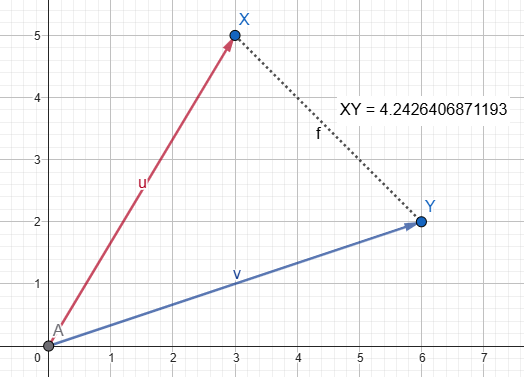
\includegraphics[width=0.7\linewidth]{EjemploEuclidiana.png}
        \caption{Representación gráfica de la Distancia Euclidiana entre dos vectores.}
        \label{fig: EjemploEuclidiana}
    \end{figure}

    \textbf{DISTANCIA DE COSENO}

    Siguiendo a \parencite{10.5555/1941884}, la Distancia del Coseno es otra de las medidas de distancia más comunes cuando un item es considerado un vector. Esta distancia se centra en calcular el coseno del ángulo a través de la \textbf{Similaridad} definida como: 
    
    \begin{equation}
        cos(x, y) = \frac{(\vec{x} \cdot \vec{y})}{|| \ \vec{x} \ || \ || \ \vec{y} \ || }
        \addequation{Definición de la Similaridad de Coseno}
        \label{SimilaridadCoseno}
    \end{equation}

    La fórmula de la Similaridad del Coseno utiliza dos cálculos algebráicos comunes en los vectores, el \textbf{\textit{Producto Punto}} y el calculo de \textbf{\textit{Norma o Magnitud}}.

    Citando a \parencite{poole2007álgebra}, el \textit{Producto Punto} se define como:

    \begin{equation}
        \begin{split}
            \vec{u} = \begin{bmatrix}
                u_1
                \\
                u_2
                \\
                \vdots
                \\
                u_n
            \end{bmatrix} &,  \ \
            \vec{v} = \begin{bmatrix}
                v_1
                \\
                v_2
                \\
                \vdots
                \\
                v_n
            \end{bmatrix}
            \\
            \\
            (u \cdot v) = u_1 v_1 + &u_2 v_2 + \hdots + u_n v_n
        \end{split}
        \addequation{Definición de Producto Punto}
        \label{eq:DefProductoPunto}
    \end{equation}

    \newpage

    Y la \textit{Norma o Magnitud} de un vector se define como el escalar no negativo $|| \ \vec{v} \ ||$ definido por: 

    \begin{equation}
        \begin{split}
            \vec{V} = &\begin{bmatrix}
                v_1
                \\
                v_2
                \\
                \vdots
                \\
                v_n
            \end{bmatrix}
            \\
            \\
            || \ \vec{V}  \ || = \sqrt{\vec{V} \cdot \vec{V}} &= \sqrt{v_1^2 + v_2^2 + \hdots + v_n^2}
        \end{split}
        \addequation{Definición de Norma o Magnitud}
    \end{equation}    

    Una vez entendiendo cómo calcular la similaridad, se calcula la distancia del coseno:
    
    \begin{equation}
        d(\vec{x}, \vec{y}) = 1 - cos(\vec{x}, \vec{y})
        \addequation{Definición de Distancia del Coseno}
    \end{equation}

    Para ilustrar la distancia del coseno mediante un ejemplo visual se definen los siguientes vectores:

    \begin{equation}
        \begin{split}
            \vec{x} &= \begin{bmatrix}
                3
                \\
                5
            \end{bmatrix},  
            \vec{y} = \begin{bmatrix}
                6
                \\
                2
            \end{bmatrix}
            \\
            \\
            || \vec{x} || &= \sqrt{3^2 + 5^2} = \sqrt{34} \approx 5.83
            \\
            || \vec{y} || &= \sqrt{6^2 + 2^2} = \sqrt{40} \approx 6.32
            \\
            \\
            ( \vec{x} \cdot \vec{y} )&=(3 \cdot  6)+(5 \cdot 2)=28
            \\
            \\
            cos(\vec{x}, \vec{y}) & = \frac{28}{5.83 \cdot 6.32} \approx 0.759
            \\
            \\
            d(\vec{x}, \vec{y}) &\approx 1 - 0.759 \approx  0.241
        \end{split}
        \addequation{Ejemplo de Distancia del Coseno}
        \label{eq:EjemploCoseno}
    \end{equation}

    \newpage

    Para entender las equivalencias entre la \Cref{fig: EjemploCoseno} y la \Cref{eq:EjemploCoseno} es importante mencionar que el calculo geométrico de la Similitud del Coseno se puede realizar mediante el calculo de $cos(\alpha)$ donde $\alpha$ representa el ángulo de separación entre $\vec{x}, \vec{y}$. Entendiendo esto, se puede visualizar que ambos resultados coinciden y representan la distancia del Coseno.

    \begin{figure}[h!]
        \centering
        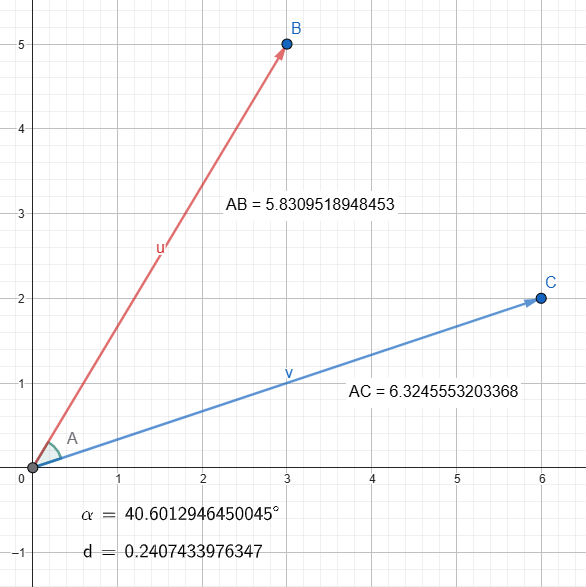
\includegraphics[width=0.7\linewidth]{EjemploCoseno.png}
        \caption{Representación gráfica de la Distancia de Coseno entre dos vectores.}
        \label{fig: EjemploCoseno}
    \end{figure}

    \textbf{PRODUCTO INTERNO}

    Según \parencite{libretexts-2024}, el \textit{Producto Interno} es un concepto extenso dentro del Álgebra Lineal, sin embargo, en el contexto de los Sistemas de Recomendación el concepto se puede reducir a una extensión del \textit{Producto Punto} de dos vectores \textbf{siempre y cuando} todos los vectores cumplan con la propiedad de pertenecer al espacio de $\mathbb{R}^n$ que, en los sistemas de recomendación, se cumple en la mayoría de casos. El \textit{Producto Interno} mide la similitud entre dos vectores y se puede calcular de la misma manera descrita en la \Cref{eq:DefProductoPunto}

    \newpage

    Para enteder cómo funciona el \textit{Producto Punto} se usará nuevamente una representación geométrica mediante los siguientes vectores:

    \begin{equation}
        \begin{split}
            \vec{x} = \begin{bmatrix}
                2
                \\
                2
            \end{bmatrix}, \
            \vec{y} &= \begin{bmatrix}
                -2
                \\
                -1
            \end{bmatrix}, \
            (\vec{x}, \vec{y}) \in \mathbb{R}^2
            \\
            \\
            (\vec{x} \cdot \vec{y}) = (2 \cdot (-2)) &+ (2 \cdot (-1)) = -4 - 2 = -6
        \end{split}
        \addequation{Ejemplo de Producto Interno}
        \label{eq:EjProductoInterno}
    \end{equation}

    En la \Cref{eq:EjProductoInterno} el resultado dado es negativo debido a que los vectores apuntan en sentidos contrarios como se puede ver en la \Cref{fig: EjemploInner}. Si el resultado obtenido fuera 0 significa que los vectores son perpendiculares y en el caso de ser positivos significa que los vectores apuntan en direcciones parecidas. Entre más alto el valor del \textit{Producto Interno} más alta la similitud de los vectores. Se debe tomar en cuenta que el valor obtenido de esta métrica no está normalizado y es afectado por la \textit{magnitud} de los vectores.

    \begin{figure}[h!]
        \centering
        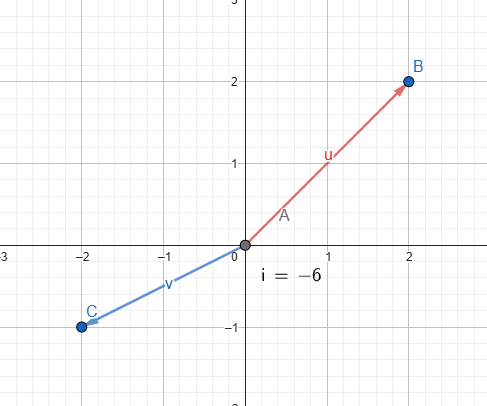
\includegraphics[width=0.7\linewidth]{EjemploInnerProduct.png}
        \caption{Representación gráfica del Producto Punto entre dos vectores.}
        \label{fig: EjemploInner}
    \end{figure}


    \newpage

    





    

\section{BÚSQUEDA DE VECINOS CERCANOS}

Uno de los métodos de búsqueda de recomendaciones más populares es el método de búsqueda de vecinos más cercanos más comunmente denominado como \text{K-Nearest Neighbors (k-NN)}. Este término es usado debido a que esta búsqueda se centra en encontrar los $k$ puntos más cercanos (o también denominados como \textit{Vecinos}) a partir de un registro de entrenamiento\parencite{10.5555/1941884}.

Se puede definir a la \textit{Búsqueda de Vecinos más cercanos} de la siguiente manera: 


\begin{definition}
    Dado un punto petición $q$ al que se le quiere conocer su clase $l$, y un conjunto de entrenamiento $X = \{ \{x_1, l_1\}\hdots\{x_n\} \}$, donde $x_j$ es el j-ésimo elemento y $l_j$ representa la etiqueta de la clase, los métodos \textit{k-NN} encuentran el subconjunto $Y = \{\{y_1, l_1\} \hdots \{y_k\} \}$ tal que $Y \in X$ y, además, $\sum^k_1d(q, y_k)$ \footnote{Representa la sumatoria de distancias entre $q$ y cada elemento $y_k \in Y$, pudiendo calcularse ya sea con distancia euclidiana, distancia de coseno o producto interno.}  se minimiza. El subconjunto $Y$ contiene los $k$ puntos en $X$ que son los más cercanos al punto petición $q$ \parencite{10.5555/1941884}.  
\end{definition}

Antes de implementar un método de \textit{Vecinos más Cercanos} es importante definir una \textit{funcion de similaridad}, según \parencite{Aggarwal2016} la más común es la \textit{Distancia de Coseno}.  Esta función de similaridad, independientemente de la elegida, cumple la función de predecir la preferencia del usuario respecto a un item que no ha evaluado. 

Una vez elegida la función de similaridad, el siguiente paso es definir el valor de $k$ que, en el punto de vista de \parencite{10.5555/1941884} es el reto más importante al usar los métodos de vecinos cercanos, debido a que un valor pequeño de $k$ incrementa la cantidad de \textit{ruido}\footnote{\textbf{Ruido}: Es definido como un error aleatorio o una varianza en una variable medida \parencite{alasadi2017review}. } en los resultados, sin embargo, si $k$ es muy grande, el vecindario podría incluir muchos puntos de diversas clases.


\section{BÚSQUEDA APROXIMADA DE VECINOS CERCANOS}

La \textit{Búsqueda Aproximada de Vecinos Cercanos (ANN)} es una de las propuestas más avanzadas de optimización para los enfoques \textit{k-NN} redefiniendo el objetivo principal para obtener resultados con taza de efectividad similar pero con un costo computacional más bajo.

\begin{definition}
    La \textit{Búsqueda aproximada de los $k$ vecinos más cercanos} se define como la búsqueda de aquellos puntos cuya distancia de la petición $q$ no excede a $(1 + \epsilon)$ 
\end{definition}

\section{INFORMACIÓN CONTEXTUAL EN LOS SISTEMAS DE RECOMENDACIÓN}

La forma en que se ha abordado el problema principal de los sistemas de recomendación ha evolucionado a lo largo del tiempo, sin embargo, la mayoría de investigaciones se enfocan en la interacción \textit{item - usuario} o \textit{usuario - item} y no se suele tomar en cuenta ningún tipo de contexto adicional que podría alterar la calidad de las recomendaciones.

Sin embargo, con la evolución de los Sistemas de Recomendación, ha surgido la necesidad de categorizar a los sistemas que son \textbf{sensibles al contexto} para encontrar métodos y enfoques que logren brindar al sistema la información necesaria para entender las necesidades y preferencias del usuario. Estos sistemas de recomendación sensibles al contexto se definen formalmente como \textit{Context-Aware recommender systems (CARS)}. 

\begin{definition}

En los sistemas de recomendación, el \textbf{Contexto} se puede definir como cualquier información que puede ser usada para caracterizar la situación de una entidad, donde una entidad puede representar a una persona, un lugar o un objeto computacional. Esta información adicional puede ayudar al sistema a ser más preciso. \mbox{\parencite{mateos2024systematic}}.

\end{definition}

Los \textit{CARS} son aquellos sistemas que buscan entender las preferencias del usuario incorporando información contextual en el proceso de recomendación. Esto implica que una calificación dada por el usuario ahora es afectada también por el contexto en el que se realizó. Por lo tanto, según \parencite{10.5555/1941884}, una \textit{calificación} ahora se puede definir de la siguiente manera:

\begin{equation}
    Usuario \times Item \times Contexto \rightarrow Calificacion
    \addequation{Cálculo de Calificación mediante un Contexto}
\end{equation}

Es importante mencionar que el Contexto puede definir diferentes aspectos del contexto del sistema ya sea tiempo, localización, compañía, propósito, y muchos más. 

\newpage

\subsection{PREFILTRADO CONTEXTUAL}

En el \textit{Prefiltrado Contextual} el contexto específico determinará qué información es la más relevante respecto a las preferencias del usuario, obteniendo un subconjunto de elementos que servirá como base para obtener recomendaciones mediante los algorítmos de recomendación clásicos.
El prefiltrado de items mediante contexto aumenta la diversidad de recomendaciones gracias a la división de datos en diferentes escenarios contextuales, sin embargo, tratar de recrear un contexto específico puede llevar a un problema de \textbf{escasez de datos}, obteniendo una recomendación altamente limitada \parencite{mateos2024systematic}.

En general, cuando se busca desarrollar un sistema de recomendación, usar un prefiltrado contextual puede resultar en desventajas importantes que afectan al desempeño del sistema, principalmente si se busca un enfoque generalizable a distintos dominios. A pesar de sus limitaciones en escenarios generales, el prefiltrado sigue siendo útil cuando se diseña en campos específicos.

\subsection{HEURÍSTICAS DE PREFILTRADO}

Para obtener un subconjunto relevante de items se suelen usar diversas técnicas de prefiltrado, una de ellas es el uso de \textbf{Heurísticas}.

\begin{definition}
    Las \textbf{Heurísticas} son criterios, métodos o principios para decidir entre diversas ramas de acción a aquella que prometa ser la más efectiva para lograr cierto propósito. Una heurística podría ser un atajo usado para guiar cierta acción \parencite{Pearl1984}.
\end{definition}

El objetivo de una Heurística no es garantizar la mejor solución a un problema, sino proponer una solución \textbf{suficientemente buena} en un tiempo razonable. En el caso de los sistemas de recomendación sensibles al contexto, las heurísticas permiten seleccionar de manera rápida un subconjunto de ítems relevantes para un usuario bajo un contexto particular, obteniendo una muestra significativa sobre el cual podrían operar los algorítmos de recomendación tradicionales.

\begin{definition}
    Los \textbf{Algorítmos Heurísticos} son una clase de algorítmos matemáticos que utilizan diversas técnicas heurísticas para la resolución de problemas complejos \parencite{proy2024algoritmos}.
\end{definition}

Las técnicas heurísticas más importantes para los algorítmos propuestos en el presente proyecto son las \textit{heurísticas voraces} y las \textit{heurísticas tabú}.

Antes de explicar de manera detallada estas heurísticas, es importante comprender el concepto de \textbf{espacio de estados} y \textbf{Funciones Heurísticas}. 

\begin{definition}
    El \textbf{espacio de estados} es el conjunto de todas las posibles configuraciones o situaciones que un sistema o problema puede alcanzar. Cada \textbf{estado} representa una situación particular del sistema, y una \textbf{transición} representa una acción o movimiento permitido con un costo asociado \parencite{heusner2017understanding}.
\end{definition}

En ciertos algorítmos el \textit{espacio de estados} es un conjunto predefinido que representa el espacio total con el que se trabajará, sin embargo, igualmente existen \textbf{modelos generativos de espacio de estados} que generan estados bajo demanda en lugar de tenerlos definidos desde el inicio. Los \textbf{modelos generativos} brindan la posibilidad de explorar \textbf{espacios grandes} sin necesidad de procesar toda la información. Estos algoritmos se apoyan en la estimación de costos o distancias entre estados para decidir cuál estado expandir en cada paso.

\begin{definition}
    Las \textbf{Funciones Heurísticas} son funciones que estiman el \textbf{costo} o \textbf{distancia} desde el estado inicial hasta el estado final \parencite{heusner2017understanding}.
\end{definition}

Las funciones heurísticas nos permiten estimar el costo o distancia entre estados mediante cálculos o procedimientos algorítmicos, sin embargo, en muchas ocasiones son llamadas \textit{cajas negras} ya que, en ciertas situaciones, no importa cómo calcula la heurística, solo importa la información que retorna.

\subsubsection{HEURÍSTICAS VORACES (GREEDY)}
Los \textit{Algorítmos Voraces} representan una estrategia para generar soluciones \textit{suboptimas} mediante ramas de decisiones irrevocables. Cada una de estas decisiones representa la mejor opción en el momento en que se toman \parencite{khuller2018greedy}.

En el ámbito de la algorítmia, los algorítmos voraces son usados para encontrar respuestas \textbf{máximas} o \textbf{mínimas} a un problema. Sin embargo, en sistemas complejos, también suelen ser usados para obtener soluciones \textbf{aproximadas} encontrando respuestas que podrían ser \textit{subóptimas} pero cumpliendo con un mínimo de rendimiento. 

A continuación se describen algunos algorítmos clásicos que utilizan heurísticas voraces para la exploración del espacio de estados.

\newpage

\textbf{ALGORÍTMO VORÁZ DE BÚSQUEDA POR NIVELES}

El \textit{Algorítmo Voráz de Búsqueda a Profundiad} o \textit{(GBFS)} es un algorítmo de búsqueda informada y voráz que intenta alcanzar la meta priorizando los estados que parecen más cercanos según la heurística, aunque no garantiza el costo mínimo total. Recibe como entrada un \textit{espacio de estados} estático o generativo y devuelve un plan que alcanza la meta sin embargo, existen casos \textit{insolubles} que indican que no se puede llegar a la meta.

Según \parencite{heusner2017understanding} la \textit{GBFS} se basa en la suposición de que los estados con menor \textbf{valor heurístico} (costo) forman parte del camino más barato hacia la meta, por esta razón se considera un \textit{algoritmo voráz}. Este algoritmo no necesita conocer todo el espacio de estados para funcionar debido a que únicamente opera en los estados que ya han sido generados. En cada paso el estado actual se expande al que tiene el \textit{menor valor heurístico} entre todos los estados que han sido generados que no han sido visitados previamente, esto se repite hasta generar el estado destino. 

Este criterio \textit{voráz} es la razón por la que este algoritmo no genera las soluciones más cortas debido a que en la mayoría de casos una decisión local no es suficiente para predecir el mejor resultado global, inclusive, no hay garantías de que el resultado tenga un mínimo de calidad. Debido a la inexactitud de la heurística, \textit{GBFS} puede quedarse atrapado en mesetas donde muchos estados tienen el mismo valor heurístico, o en mínimos locales donde la heurística guía hacia caminos no óptimos, lo que puede aumentar el tiempo de búsqueda o producir soluciones subóptimas.

\begin{figure}[h!]
    \centering
    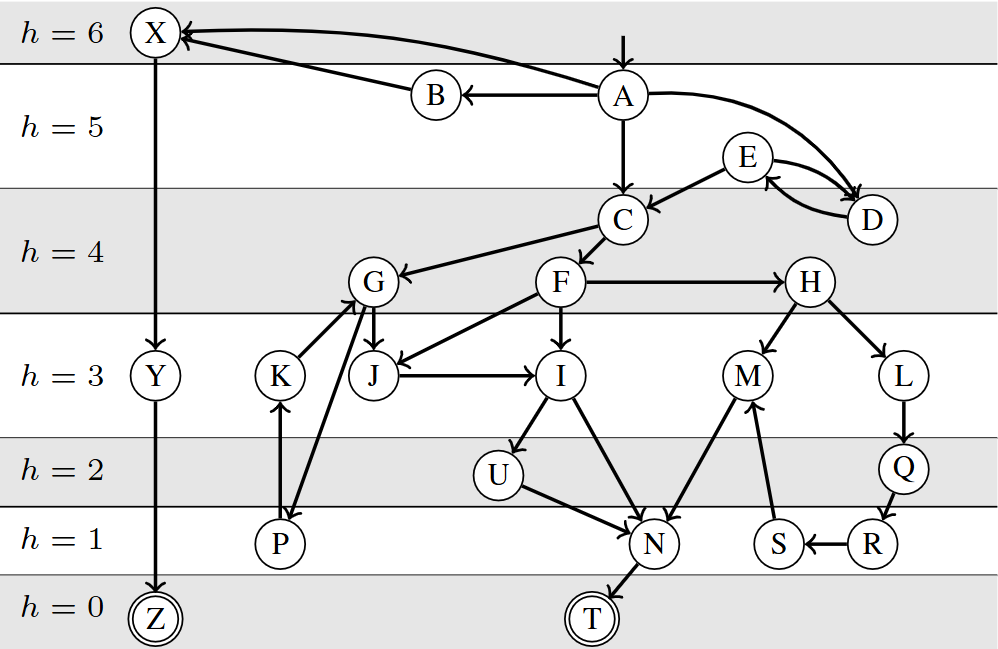
\includegraphics[width=0.7\linewidth]{EjemploDeGBFS.png}
    \caption{Ejemplo de GBFS \parencite{heusner2017understanding}.}
    \label{fig:EjemploGBFS}
\end{figure}

En la \Cref{fig:EjemploGBFS} se define el estado inical el nodo $A$ y el nodo objetivo $Z$. Cada nivel horizontal indica el cálculo $h$ de la distancia mediante la \textit{función heurística}. Además, se puede ver que existen diferentes caminos para llegar al nodo $Z$ y \textit{GBFS} podría retornar un camino menos óptimo como el más prometedor.

\textbf{ALGORITMO DE BÚSQUEDA A*}

El algoritmo \textit{A*} es un algoritmo que aprovecha una \textit{función heurística} para guiar su búsqueda hacia el nodo objetivo. Este algoritmo combina los mejores aspectos del \textit{Algoritmo Dijkstra}\footnote{\textbf{Algoritmo Dijkstra:} Algoritmo que encuentra el camino más corto a todos los nodos desde un único nodo orígen \parencite{javaid2013understanding}.} y \textit{GBFS} \parencite{KumarRAStar}. Esta combinación de algorítmos se puede definir de manera formal mediante la combinación de funciones $g(n)$ que representa el costo o distancia para alcanzar el nodo $n$ desde el nodo inicial, y $h(n)$ el costo de llegar desde un nodo $n$ hasta el nodo destino:

\begin{equation}
    f(n) = g(n) + h(n)
    \addequation{Definición de la función de A*}
\end{equation}

Así, $f(n)$ representa el costo estimado de la solución más barata que pase por el nodo $n$. Por lo tanto, si se busca encontrar la solución más barata, la estrategia es priorizar el nodo con el valor mínimo de $g(n) + h(n)$. Esta combinación es razonable y, junto a una buena \textit{función de heurística}, la \textit{búsqueda A*} garantiza soluciones óptimas \parencite{RusselArtificialIntelligence}. 

\begin{figure}[h!]
    \centering
    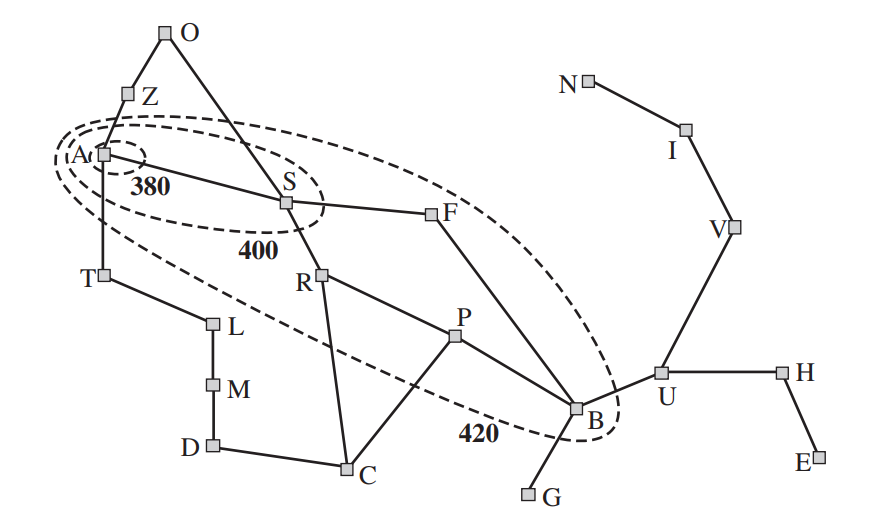
\includegraphics[width=0.8\linewidth]{EjemploASearch.png}
    \caption{Ejemplo del Algoritmo A* \parencite{RusselArtificialIntelligence}.}
    \label{fig:EjemploAStar}
\end{figure}

\newpage

En la \Cref{fig:EjemploAStar} se representa un problema clásico de inteligencia artíficial usado para explicar el algoritmo \textit{A*} llamado \textit{El Mapa de Rumanía}. Cada nodo representa una ciudad de Rumanía y las conexiones entre nodos representan las carreteras entre ciudades. El problema pide encontrar la ruta más corta desde \textit{Arad} hasta \textit{Bucarest}. En los contornos se muestran los valores $f(x)$ de los nodos que representan el camino más corto desde el inicio.

\subsubsection{HEURÍSTICAS TABÚ}




